\documentclass[conference]{IEEEtran}
\IEEEoverridecommandlockouts
\usepackage{cite}
\usepackage{amsmath,amssymb,amsfonts}
\usepackage{algorithmic}
\usepackage{graphicx}
\usepackage{textcomp}
\usepackage{xcolor}
\usepackage{subfigure}
\usepackage{multirow}
\usepackage[UTF8]{ctex}
\def\BibTeX{{\rm B\kern-.05em{\sc i\kern-.025em b}\kern-.08em
    T\kern-.1667em\lower.7ex\hbox{E}\kern-.125emX}}

\newcommand\blfootnote[1]{%
  \begingroup
  \renewcommand\thefootnote{}\footnote{#1}%
  \addtocounter{footnote}{-1}%
  \endgroup
}

\begin{document}

\title{基于通信协作的多追逐者非线性追逃博弈协同策略}

\author{
\IEEEauthorblockN{高悠然}
\IEEEauthorblockA{\textit{计算机学院} \\
\textit{北京航空航天大学}\\
北京 100191 \\
gaoyouran@buaa.edu.cn}
\and
\IEEEauthorblockN{张坤}
\IEEEauthorblockA{\textit{宇航学院} \\
\textit{北京航空航天大学}\\
北京 100191 \\
zhangkun22@buaa.edu.cn}
}

\maketitle

\begin{abstract}
多追逐者追逃博弈广泛出现在无人机编队拦截等实际场景中，需要在非线性动力学和执行器饱和约束下实现团队协同捕获。
现有方法基于Hamilton--Jacobi--Isaacs (HJI)方程为每个追逐者独立求解最优控制策略，能够产生有效的个体追踪策略，但忽略了队友之间的空间关系。
当多个追逐者指向同一逃逸者时，这种解耦求解方式倾向于产生相似的接近轨迹，限制了追逐团队的空间多样性。
本文提出一种基于追逐者间通信的轻量级协调机制：每个追逐者通过通信图从队友处获取位置信息，据此计算排斥梯度并与学习到的值函数梯度在饱和控制律内部叠加。
由于协调信号是加性的且不改变训练过程，该框架保持了原始学习算法的收敛性，并在通信丢失时自然退化为基线策略。
在六自由度非线性飞行器模型上，对从三追一到八追四的五种团队配置进行了仿真验证。
实验表明所提方法能够有效分散接近路径而不影响捕获性能，并且在30\%丢包率下仍然有效。
\end{abstract}

\begin{IEEEkeywords}
追逃博弈、多智能体协作、通信图、强化学习、非线性控制
\end{IEEEkeywords}

\blfootnote{
本工作受国家自然科学基金项目(62103408)资助。
*通讯作者：张坤。
}

% =====================================================================
\section{引言}
% =====================================================================

协同追逃博弈是多智能体系统中的基本问题，在无人机空中拦截\cite{b_zhang2023}、卫星对抗\cite{b_gong2020}、边界防御\cite{b_shishika2020}和搜救任务等领域具有广泛的应用价值\cite{b_isaacs,b_chen2016,b_yan2022}。
这些应用通常涉及非线性飞行动力学和执行器饱和约束，使得经典线性方法不再适用，需要借助基于HJI方程的近似最优方法\cite{b_lopez2020,b_lewis1998}。

强化学习(RL)为近似求解HJI方程提供了数据驱动的路径。
其中，值函数单网络自适应评价(V-SNAC)架构直接从值函数梯度推导控制策略，无需单独的actor网络，降低了计算负担\cite{b_vsnac_ref}。
基于图论的逐对交换动态目标分配也被证明能改善多逃逸者场景中的团队内聚性\cite{b_graphswap}。
近年来，MADDPG\cite{b_maddpg}和通信感知架构\cite{b_commrl2025}等多智能体RL框架探索了集中训练分散执行的范式，但通常需要专用通信模块且随智能体数量增长扩展性较差。

逐追逐者HJI求解的一个实际局限在于：每个智能体的控制仅依赖自身相对于指派逃逸者的追踪误差。
当多个追逐者从相似初始条件出发追踪同一逃逸者时，值函数梯度指向相似方向，轨迹趋向同一条接近路径。
我们将这一现象称为\textbf{路径退化}，它源于解耦值函数结构的内在特性。

路径退化带来两个不利后果：
一是降低了追逐团队的有效空间覆盖——冗余的接近角度使逃逸方向缺乏封堵；
二是在物理部署中飞行器间过于接近的轨迹增加了冲突风险，这在协同飞行操作中是公认的安全关切\cite{b_icao_separation,b_collision_uav}。

与此相关的研究包括：基于图拉普拉斯的共识编队控制\cite{b_ren2005,b_olfati2004}、图博弈\cite{b_lopez2020,b_graphgame2023}、控制壁障函数\cite{b_ames2017}、加权拓扑协同追踪\cite{b_zhou2024}以及与RL结合的编队围捕控制\cite{b_formrl2024}。
然而，将这些机制直接嵌入具有执行器饱和的非线性HJI框架仍然技术复杂，往往需要同时重新设计代价泛函和学习过程。

本文采取不同思路：不修改训练过程，而是在执行时为控制律增加基于通信的协调梯度，以鼓励队友间的空间多样性。主要贡献包括：
\begin{itemize}
\item 提出增广控制律，在通信图上引入排斥梯度，保持HJI推导的$\tanh$饱和策略形式不变。
\item 分析表明训练收敛性不受影响，通信丢失导致向基线策略的优雅退化。
\item 在六自由度非线性飞行器模型的五种团队配置上给出仿真结果，包括直接展示路径退化及其消除的受控场景。
\end{itemize}

本文其余部分组织如下：第二节介绍系统模型、代价泛函和基线V-SNAC控制；第三节提出通信增广框架并讨论其性质；第四节给出仿真结果；第五节给出结论。


% =====================================================================
\section{预备知识}
% =====================================================================

\subsection{智能体动力学}

考虑由$N_p$个追逐者和$N_e$个逃逸者（$N_p \geq N_e$）参与的追逃博弈。
每个智能体服从控制仿射动力学：
\begin{equation}\label{eq:dynamics}
\dot{x}_j = f(x_j) + g(x_j)\,u_j, \quad \|u_j\| \leq \bar{u}
\end{equation}
其中$x_j = [p_j^T, v_j^T]^T \in \mathbb{R}^n$为包含位置和速度的状态，$u_j \in \mathbb{R}^m$为受饱和约束的控制输入，$f$和$g$均Lipschitz连续。

输入矩阵$g$具有以下结构：
\begin{equation}\label{eq:g_struct}
g(x) = \begin{bmatrix} 0_{3\times 3} \\ G_v(x) \end{bmatrix}
\end{equation}
其中$G_v \approx I_3$是状态相关的，反映了控制输入作用于加速度层。
这意味着经$g^T$传递的梯度必须在速度分量上非零才能产生实际效果。


\subsection{代价泛函与HJI方程}

追逐者$j$通过二部目标图指派到逃逸者$\sigma(j)$。追踪误差定义为：
\begin{equation}\label{eq:error}
\tilde{x}_j = x_j^p - x_{\sigma(j)}^e + r_{j,\sigma(j)}
\end{equation}
其中$r_{j,\sigma(j)}$编码围捕编队的期望偏移。零和代价泛函为：
\begin{equation}\label{eq:cost}
J_j = \int_0^\infty \!\Big[\tilde{x}_j^T Q\,\tilde{x}_j + U(u_j^p) - W(u_e)\Big]\,dt
\end{equation}
其中$Q \succ 0$惩罚追踪误差，非二次项
\begin{equation}\label{eq:nq}
U(u) = \sum_{l=1}^m 2\bar{u}\,R_{1,l}\int_0^{u_l/\bar{u}} \bar{u}\,\mathrm{arctanh}(\tau)\,d\tau
\end{equation}
确保最优控制自然满足饱和约束\cite{b_vsnac_ref}。

\subsection{V-SNAC最优控制}

鞍点值函数$V_j^* = \min_{u_j^p}\max_{u_e} J_j$满足HJI方程，由此推导出最优追逐者控制：
\begin{equation}\label{eq:ctrl_base}
u_j^{p*} = -\bar{u}_p\,\tanh\!\bigg(\frac{1}{2\bar{u}_p}\,R_1^{-1}\,g_j^T\,\nabla V_j^*\bigg)
\end{equation}
在V-SNAC框架中，$V_j$被近似为：
\begin{equation}\label{eq:vsnac}
\hat{V}_j(\tilde{x}_j) = \hat{W}_j^T\,\psi(\tilde{x}_j)
\end{equation}
其中$\psi\!:\!\mathbb{R}^n\!\to\!\mathbb{R}^h$为固定基函数，$\hat{W}_j \in \mathbb{R}^h$为可训练权重。
梯度可解析计算为$\nabla \hat{V}_j = (\nabla\psi)^T \hat{W}_j$，每个追逐者仅需一个critic网络\cite{b_vsnac_ref}。

权重通过带衰减学习率的离策略梯度下降更新：
\begin{equation}\label{eq:weight_update}
\hat{W}_{j,s+1} = \hat{W}_{j,s} - \alpha_s\,e_{j,s}\,K_{j,s}^T
\end{equation}
其中$e_{j,s}$为Bellman残差，$K_{j,s} = \nabla\psi \cdot F_j$编码漂移动力学，衰减学习率$\alpha_s = \alpha_0\,\lambda^s$确保稳定收敛\cite{b_lewis1998}。

\subsection{路径退化问题}

由于控制律\eqref{eq:ctrl_base}仅依赖$\tilde{x}_j$，分配到同一逃逸者且具有相似追踪误差的两个追逐者会产生相似控制。
在极限情况$\tilde{x}_j = \tilde{x}_k$下，控制在每一步都完全一致，轨迹完全重合。
这一解耦结构的内在特性促使我们通过追逐者间通信引入协调机制。


% =====================================================================
\section{通信增广控制}
% =====================================================================

\subsection{组内通信图}

在追踪同一逃逸者的追逐者之间定义通信图$\mathcal{G}_p = (\mathcal{V}_p,\mathcal{E}_p)$：
\begin{equation}\label{eq:adj}
a_{jk} = \begin{cases} 1, & \sigma(j) = \sigma(k),\; j \neq k \\ 0, & \text{其他} \end{cases}
\end{equation}
度$d_j = \sum_k a_{jk}$为通信伙伴数量。组内限制确保协调仅作用于轨迹有重叠风险的智能体之间。

\subsection{协调梯度}

给定图邻居的位置信息$p_k$，追逐者$j$计算基于排斥的协调梯度：
\begin{equation}\label{eq:coord_grad}
\nabla_{\mathrm{c},j} = \frac{\gamma}{d_j}\sum_{k:\,a_{jk}>0} \frac{p_j - p_k}{\|p_j - p_k\|(\|p_j - p_k\| + \epsilon)}
\end{equation}
其中$\gamma > 0$为协调强度，$\epsilon > 0$防止奇异。
梯度嵌入在状态向量的速度子空间中，以确保经$g_j^T$传递到控制律。

增广控制律为：
\begin{equation}\label{eq:ctrl_aug}
u_j^{p*} = -\bar{u}_p\,\tanh\!\bigg(\frac{1}{2\bar{u}_p}\,R_1^{-1}\,g_j^T\big[\nabla \hat{V}_j + \nabla_{\mathrm{c},j}\big]\bigg)
\end{equation}

由于两项都出现在$\tanh$内部，执行器约束$\bar{u}_p$始终被满足。
当$\gamma = 0$或$d_j = 0$时，退化为基线控制律\eqref{eq:ctrl_base}。

\subsection{增广控制的性质}

\textit{退化消除}：即使$\nabla \hat{V}_j = \nabla \hat{V}_k$（相同追踪情况），协调梯度沿$p_j - p_k$方向反平行，产生相反修正使轨迹分离。

\textit{训练不变性}：权重$W_j$在$\gamma = 0$下训练。协调梯度仅在执行时激活，离策略学习过程及其UUB收敛保证不受影响\cite{b_lewis1998}。这也允许在运行时调整$\gamma$而无需重新训练。

\textit{优雅退化}：通信丢失时边从$\mathcal{G}_p$中移除，协调梯度成比例减小。完全丢失时$\nabla_{\mathrm{c},j} = 0$，恢复基线策略。对于部分丢失（丢包率$p_d$），控制偏差有界：
\begin{equation}\label{eq:dropout}
\|u_j^{\text{full}} - u_j^{\text{drop}}\| \leq \gamma\,\|R_1^{-1}\|\,\|G_v\|_\infty\,\|\nabla_{\mathrm{c},j}^{\text{full}} - \nabla_{\mathrm{c},j}^{\text{drop}}\|
\end{equation}

% =====================================================================
\section{实验与结果分析}
% =====================================================================

\subsection{飞行器模型与参数}

所有实验使用六自由度非线性飞行器模型，状态$x = [p_x, p_y, h, v_x, v_y, v_h]^T$，控制输入$u \in \mathbb{R}^3$（加速度）。
漂移动力学包括气动力（推力、阻力、升力、俯仰力矩），采用指数衰减大气密度和攻角相关系数。
执行器饱和$\bar{u}_p = 25$（追逐者），$\bar{u}_e = 15$（逃逸者）。

V-SNAC使用每个critic $h = 6$个多项式基函数：
\begin{equation}\label{eq:basis}
\psi(\tilde{x}) = \text{gain}\cdot\big[p_1 v_1,\; p_2 v_2,\; p_3 v_3,\; \tfrac{1}{2}v_1^2,\; \tfrac{1}{2}v_2^2,\; \tfrac{1}{2}v_3^2\big]^T
\end{equation}
其中$(p_1,p_2,p_3)$为缩放后的位置误差分量，$(v_1,v_2,v_3)$为速度误差分量。
训练运行50--56轮策略迭代，学习率$\alpha_s = 0.05 \times 0.85^s$。
多逃逸者场景中启用逐对交换动态目标分配。

五种团队配置：3追1、3追3、5追3、6追3、8追4。
同一组训练权重在三种模式下评估：\textbf{全通信}（$\gamma = 0.3$）、\textbf{无通信}（$\gamma = 0$）、\textbf{丢包}（$\gamma = 0.3$，15\%逐步边移除）。

\subsection{路径退化演示}

\begin{figure}[htbp]
\centerline{
\includegraphics[width=\linewidth]{paper_figures/fig_collision_comparison.png}}
\caption{路径退化场景。左：无通信时两追逐者轨迹完全重合。中：有通信（$\gamma{=}5$）时轨迹分离。右：追逐者间距随时间变化。}
\label{fig:collision}
\end{figure}

首先隔离退化现象。两个追逐者从相近位置出发，具有相同目标位移（$r_1 = r_2$）和相同初速度。
在基线下，追踪误差和控制在每一步都相等，轨迹完全重合。
表~\ref{tab:collision}报告了追逐者间距随$\gamma$的变化。
$\gamma = 0$时路径重合；任何正$\gamma$都将它们分离，间距随$\gamma$单调增长直至饱和。
图~\ref{fig:collision}展示了轨迹和间距时间曲线。

\begin{table}[htbp]
\renewcommand\arraystretch{1.2}
\caption{路径重合测试：追逐者间距 vs $\gamma$}
\label{tab:collision}
\begin{center}
\begin{tabular}{c|cccccc}
\hline
$\gamma$ & 0 & 0.5 & 1.0 & 2.0 & 5.0 & 10.0 \\
\hline
间距 & 0.00 & 0.96 & 1.44 & 2.00 & 2.00 & 2.00 \\
\hline
\end{tabular}
\end{center}
\end{table}


\subsection{多场景结果}

表~\ref{tab:results}汇总了五种团队配置在三种通信模式下的捕获时间。

\begin{table}[htbp]
\renewcommand\arraystretch{1.2}
\caption{各团队配置的捕获时间（秒）}
\label{tab:results}
\begin{center}
\begin{tabular}{c|ccc|c}
\hline
\textbf{场景} & \textbf{全通信} & \textbf{无通信} & \textbf{丢包} & $N_p / N_e$ \\
\hline
3追1 & 55.1 & 47.2 & 53.9 & 3 \\
3追3 & 33.5 & 33.5 & 33.5 & 1 \\
5追3 & 36.5 & 36.5 & 36.5 & 1--2 \\
6追3 & \textbf{36.6} & 37.5 & 36.8 & 2 \\
8追4 & 37.9 & 36.9 & 37.6 & 2 \\
\hline
\end{tabular}
\end{center}
\end{table}

在3追1场景中，全通信增加约8秒捕获时间。这是追逐者/逃逸者比率最高的配置，协调梯度影响最大，增量反映了空间多样性与激进追击之间的权衡。

对于多逃逸者的较大团队（5追3、6追3、8追4），捕获时间差异在1秒以内。值得注意的是，6追3配置下通信模式捕获更快（36.6秒 vs 37.5秒）。一个合理的解释是分散的接近角度减少了包围阶段的相互干扰，使目标交换算法能找到更高效的分配方案。

3追3充当天然对照组：每个逃逸者仅被一个智能体追踪，组内无边（$d_j = 0$），三种模式结果完全相同。

在15\%随机丢包下，捕获时间与全通信偏差不超过0.3秒，确认部分丢失成比例减小协调梯度而不破坏追踪策略。


\subsection{场景一：三追一}

\begin{figure}[htbp]
\centerline{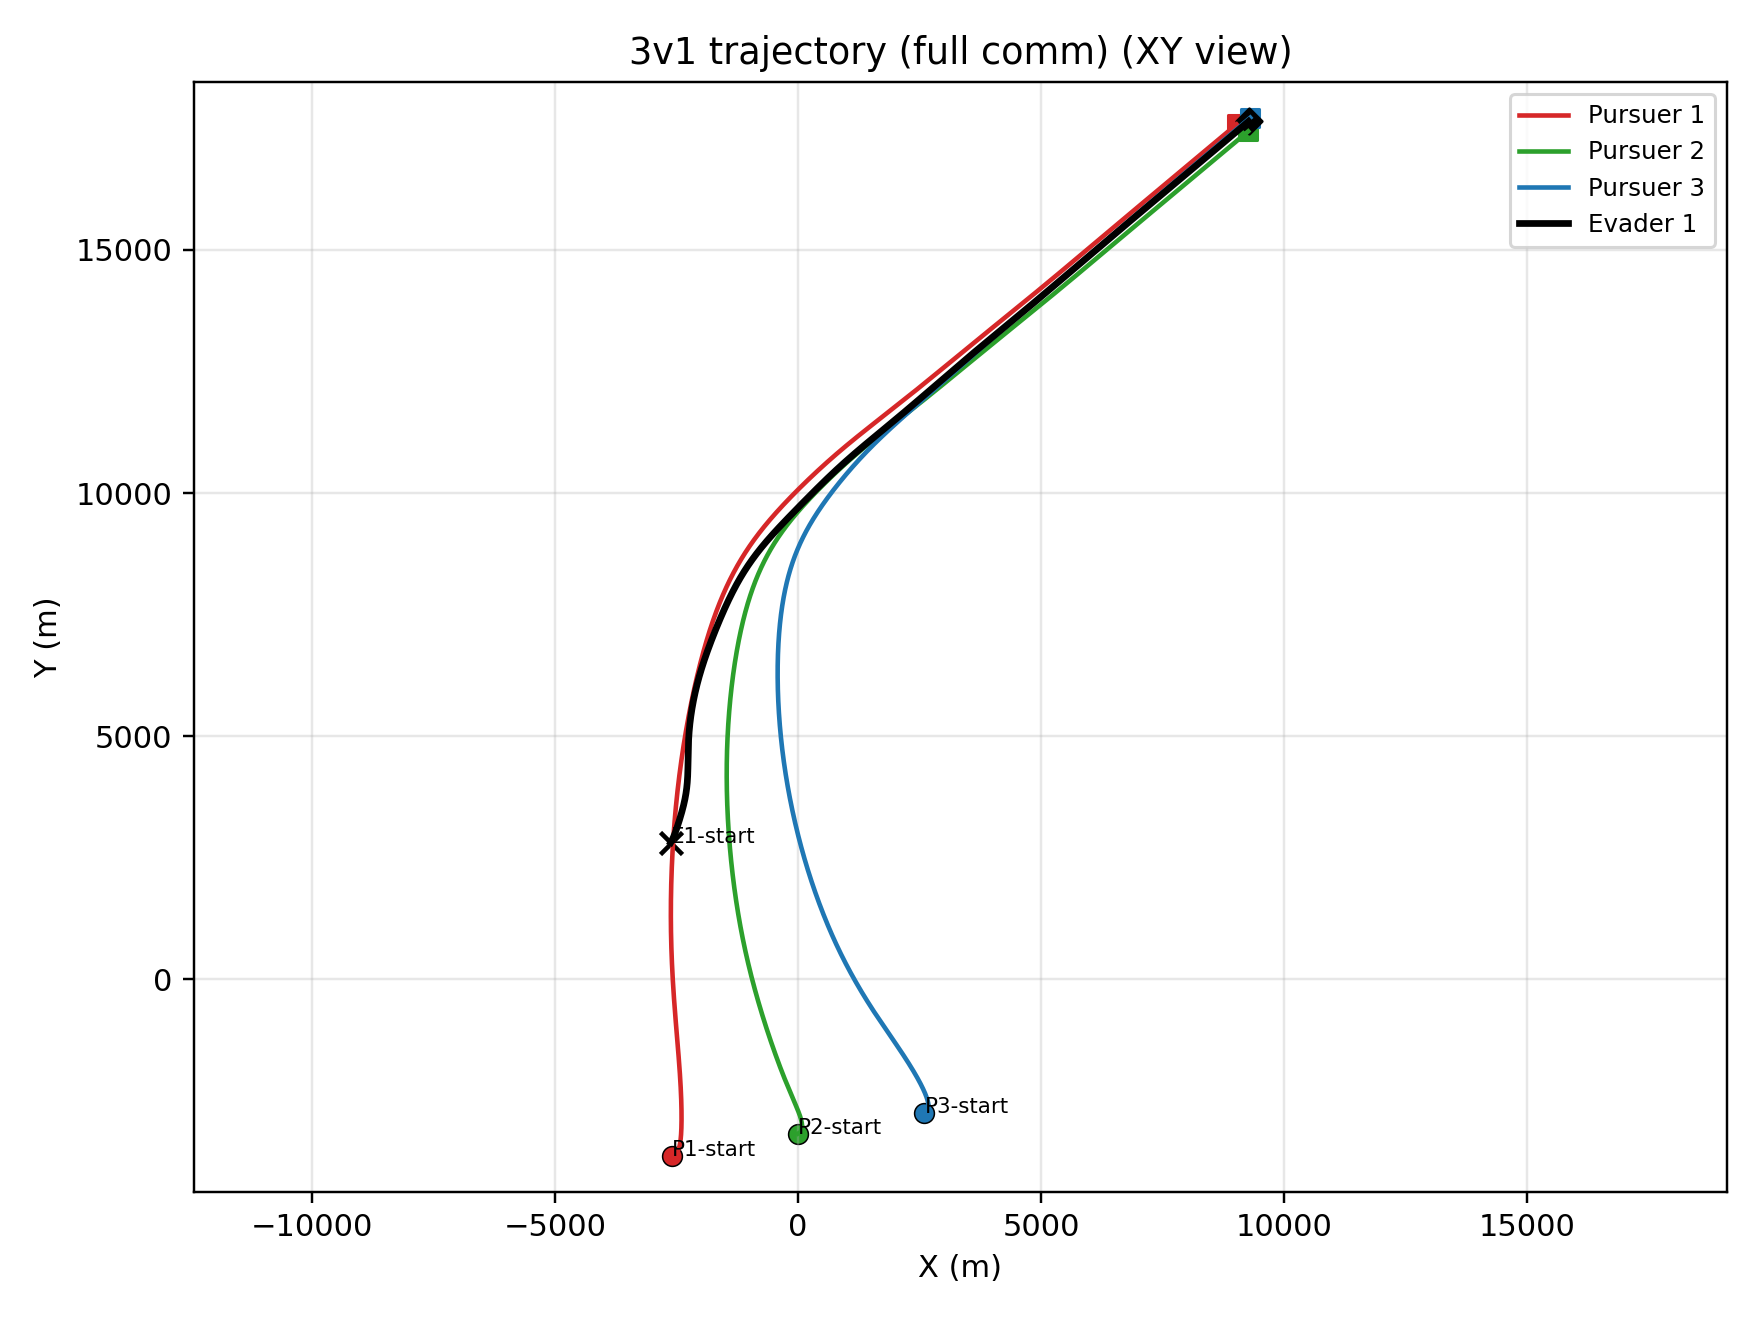
\includegraphics[width=\linewidth]{paper_figures/fig_trajectory_xy.png}}
\caption{3追1全通信轨迹。三个追逐者从不同方向接近逃逸者（黑色）。}
\label{fig:traj_3v1}
\end{figure}

\begin{figure}[htbp]
\centerline{
\includegraphics[width=\linewidth]{paper_figures/fig_assigned_errors.png}}
\caption{3追1追踪误差范数。所有追逐者收敛到小邻域，符合UUB稳定性。}
\label{fig:err_3v1}
\end{figure}

3追1场景代表协调需求最高的情况（$N_p/N_e = 3$）。图~\ref{fig:traj_3v1}显示三个追逐者在全通信下从分散方向接近逃逸者。图~\ref{fig:err_3v1}确认所有追踪误差从约7000收敛到约100的有界邻域。误差未精确趋零，因为逃逸者持续机动且V-SNAC近似带有残差界。

\begin{figure}[htbp]
\centerline{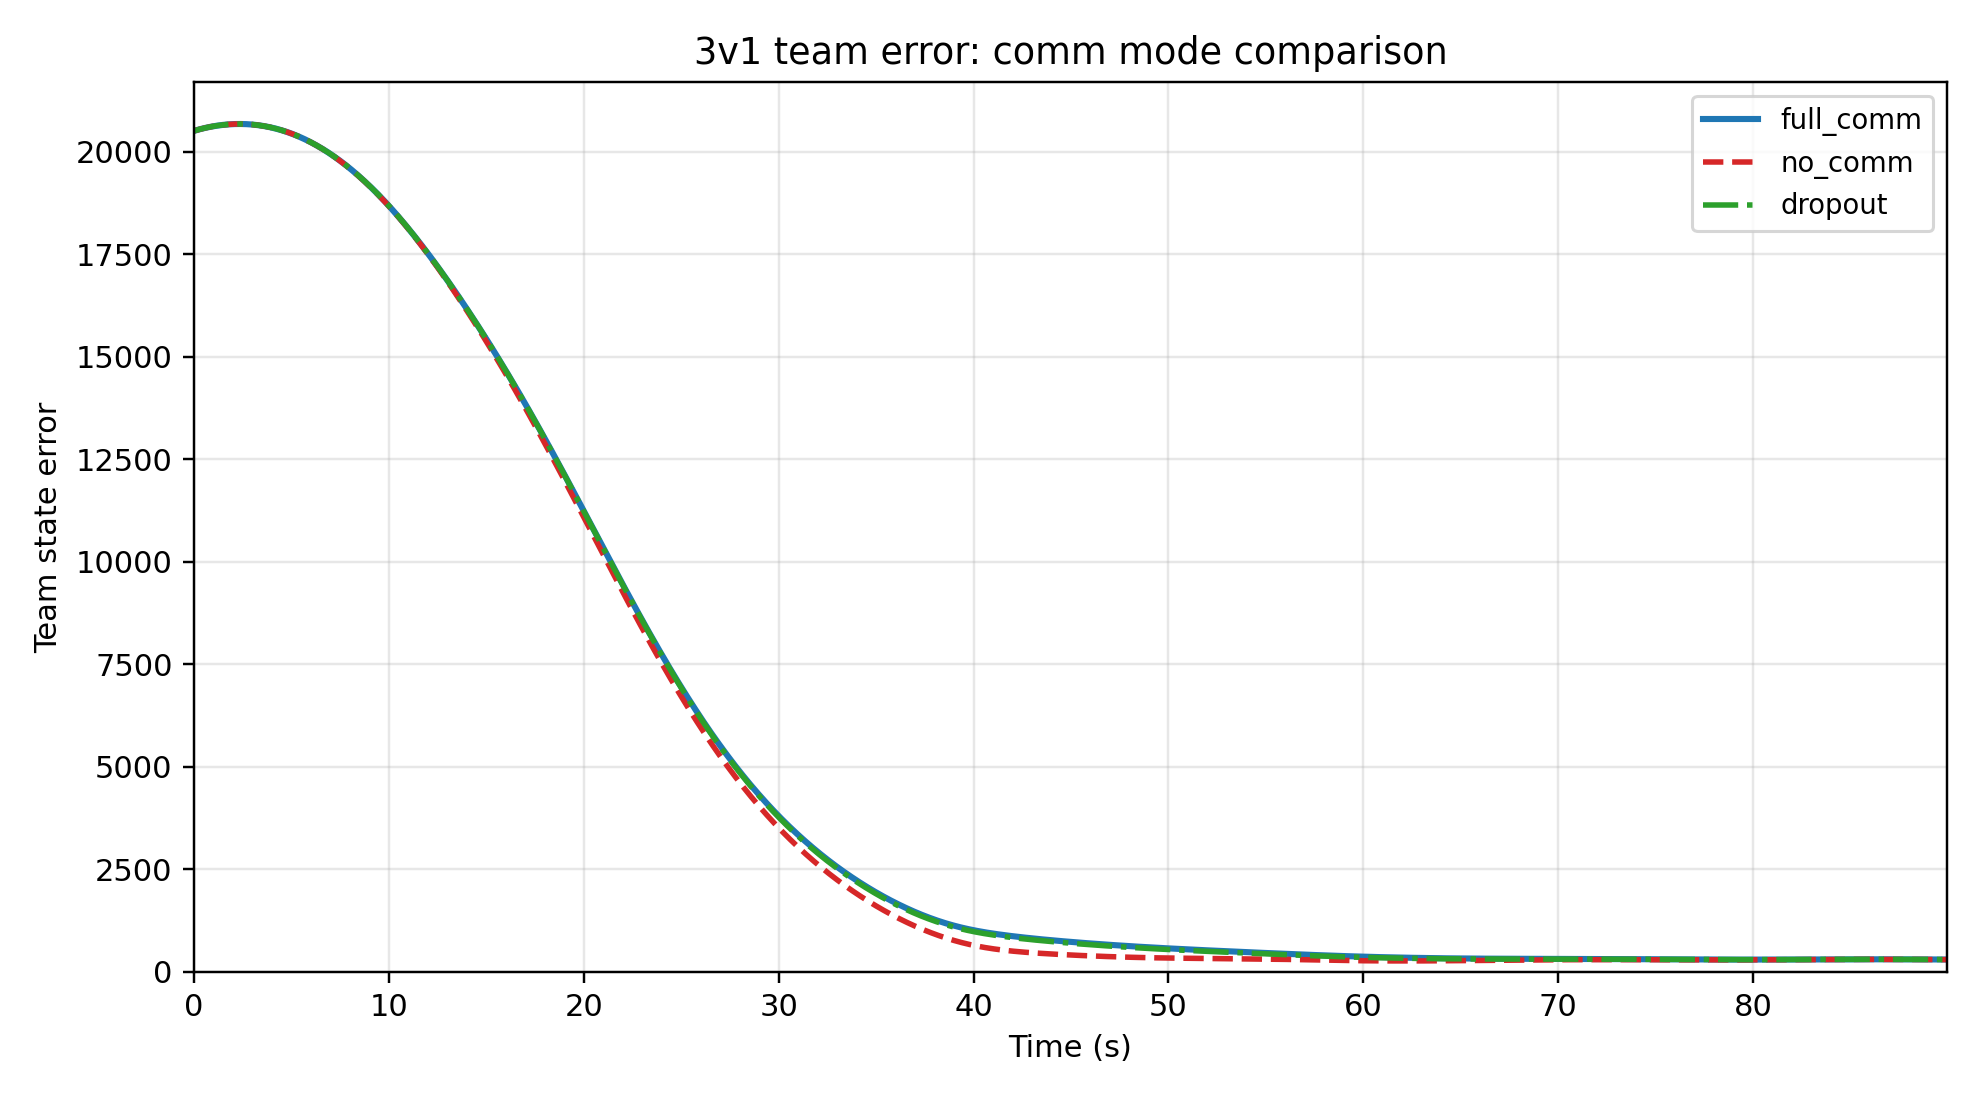
\includegraphics[width=\linewidth]{paper_figures/fig_comm_comparison.png}}
\caption{3追1三种通信模式的团队状态误差。曲线重叠，确认协调不损害追踪性能。}
\label{fig:comm_compare}
\end{figure}

图~\ref{fig:comm_compare}叠加了三种模式的团队状态误差$E_{\text{team}}$。曲线几乎完全重合，确认协调梯度不影响总体追踪性能。丢包曲线与全通信曲线无法区分。


\subsection{场景二：六追三}

\begin{figure}[htbp]
\centerline{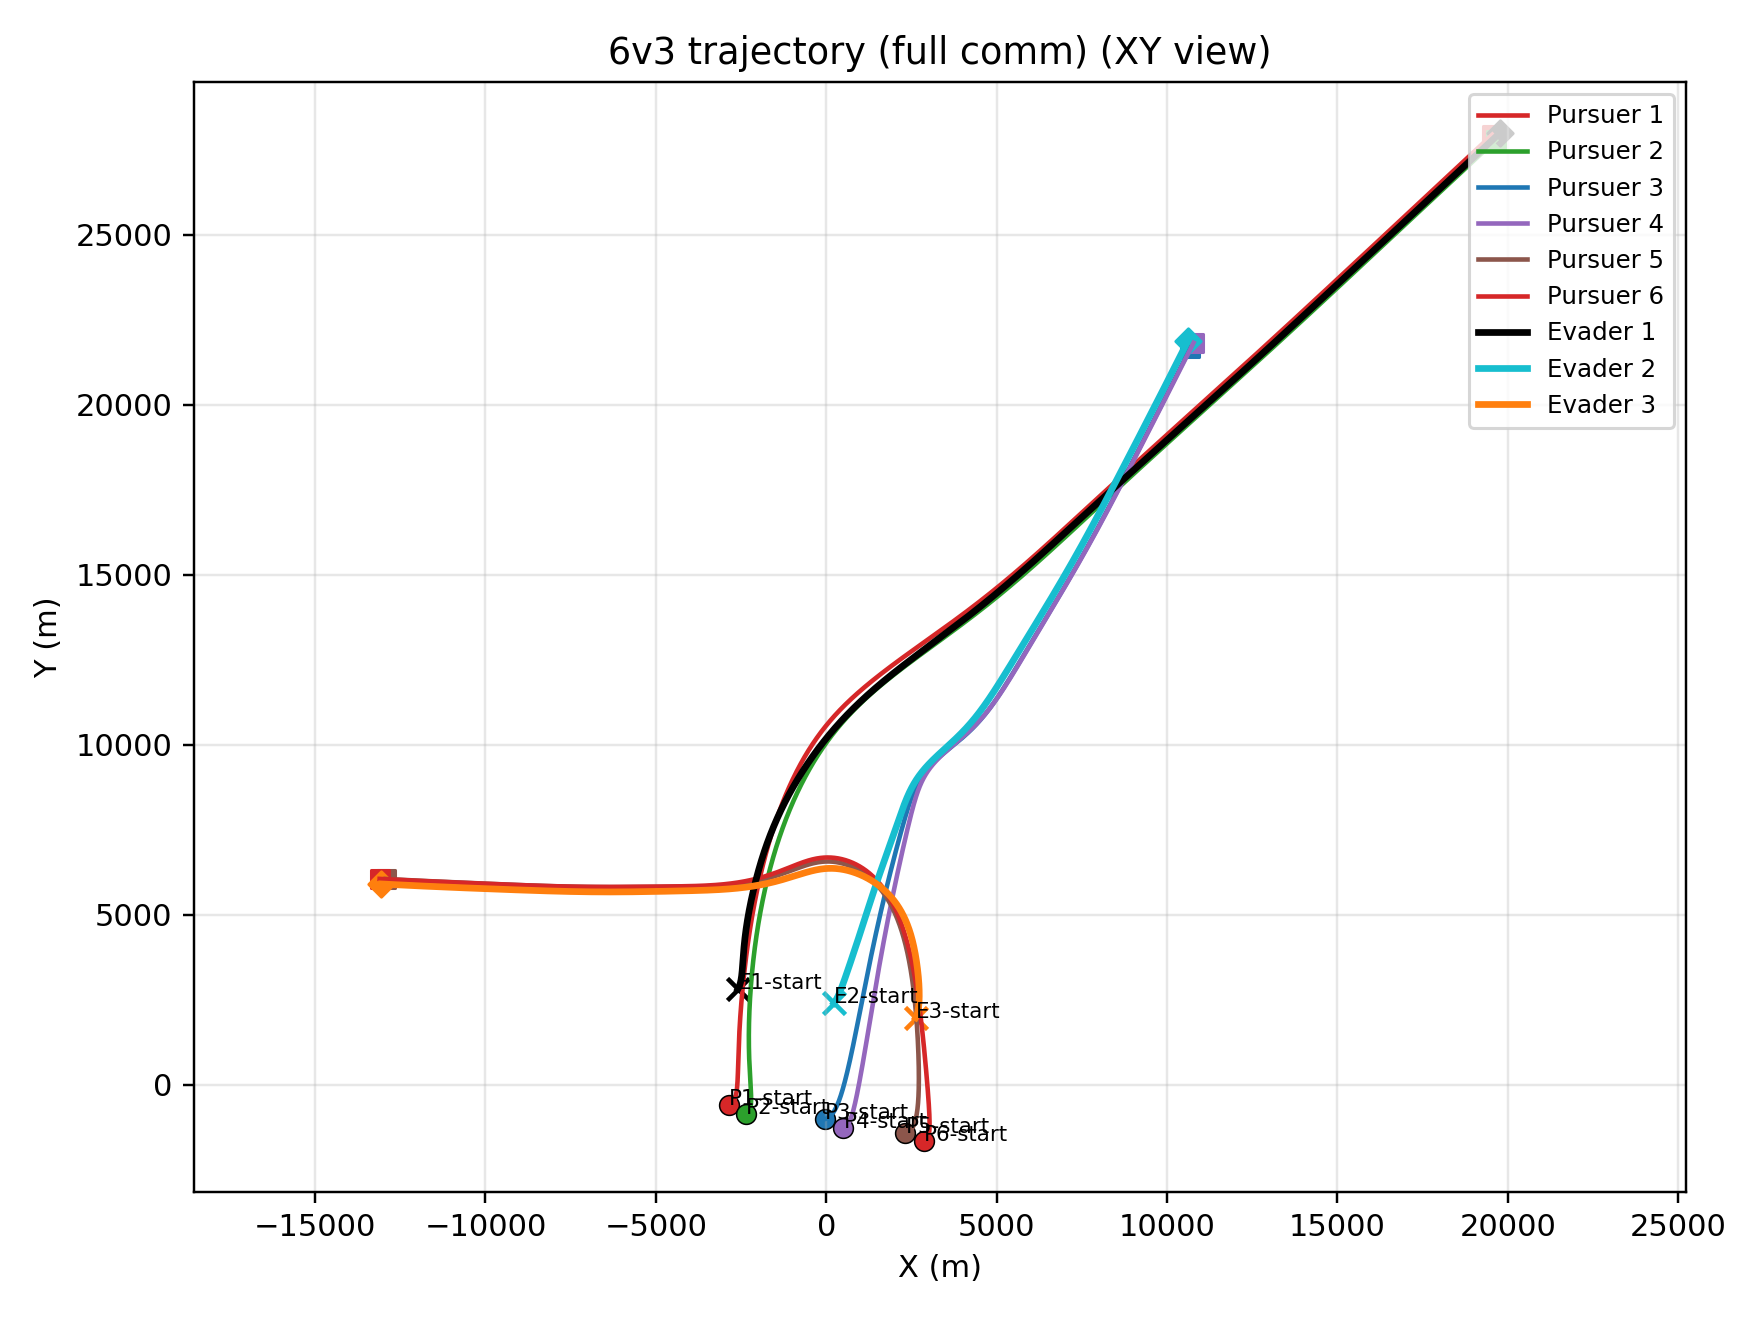
\includegraphics[width=\linewidth]{paper_figures/fig_trajectory_6v3.png}}
\caption{6追3全通信轨迹。六个追逐者（彩色）追踪三个逃逸者（深色线），伴随动态目标重分配。}
\label{fig:traj_6v3}
\end{figure}

\begin{figure}[htbp]
\centerline{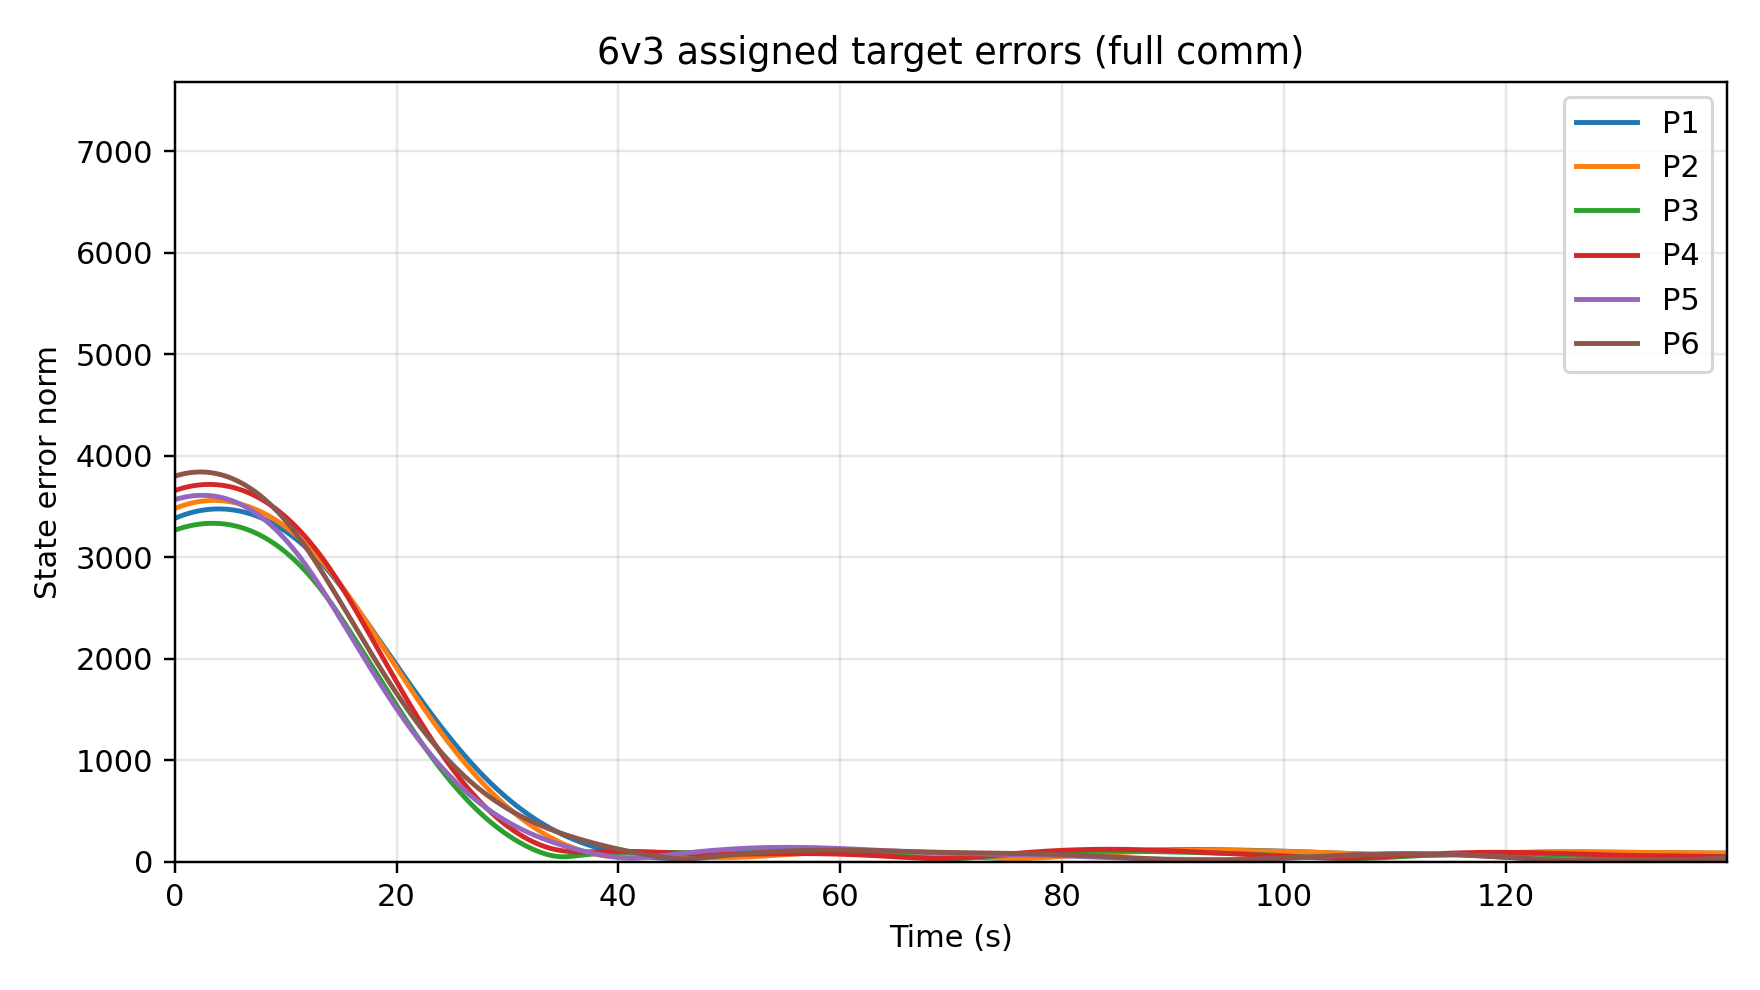
\includegraphics[width=\linewidth]{paper_figures/fig_errors_6v3.png}}
\caption{6追3追踪误差范数。所有六个追逐者收敛，$t \approx 15$秒处的斜率变化对应目标重分配事件。}
\label{fig:err_6v3}
\end{figure}

6追3结合了多逃逸者与组内协调（$N_p/N_e = 2$）。图~\ref{fig:traj_6v3}展示了更复杂的追逐几何。图~\ref{fig:err_6v3}显示所有六个追踪误差收敛，$t \approx 15$秒处的斜率变化对应目标重分配。

如表~\ref{tab:results}所示，6追3通信模式捕获略快于基线（36.6秒 vs 37.5秒）。图~\ref{fig:team_6v3}比较了动态与固定目标图下的团队状态误差，动态分配始终降低总体误差——这一效果与通信协调互补且独立。

\begin{figure}[htbp]
\centerline{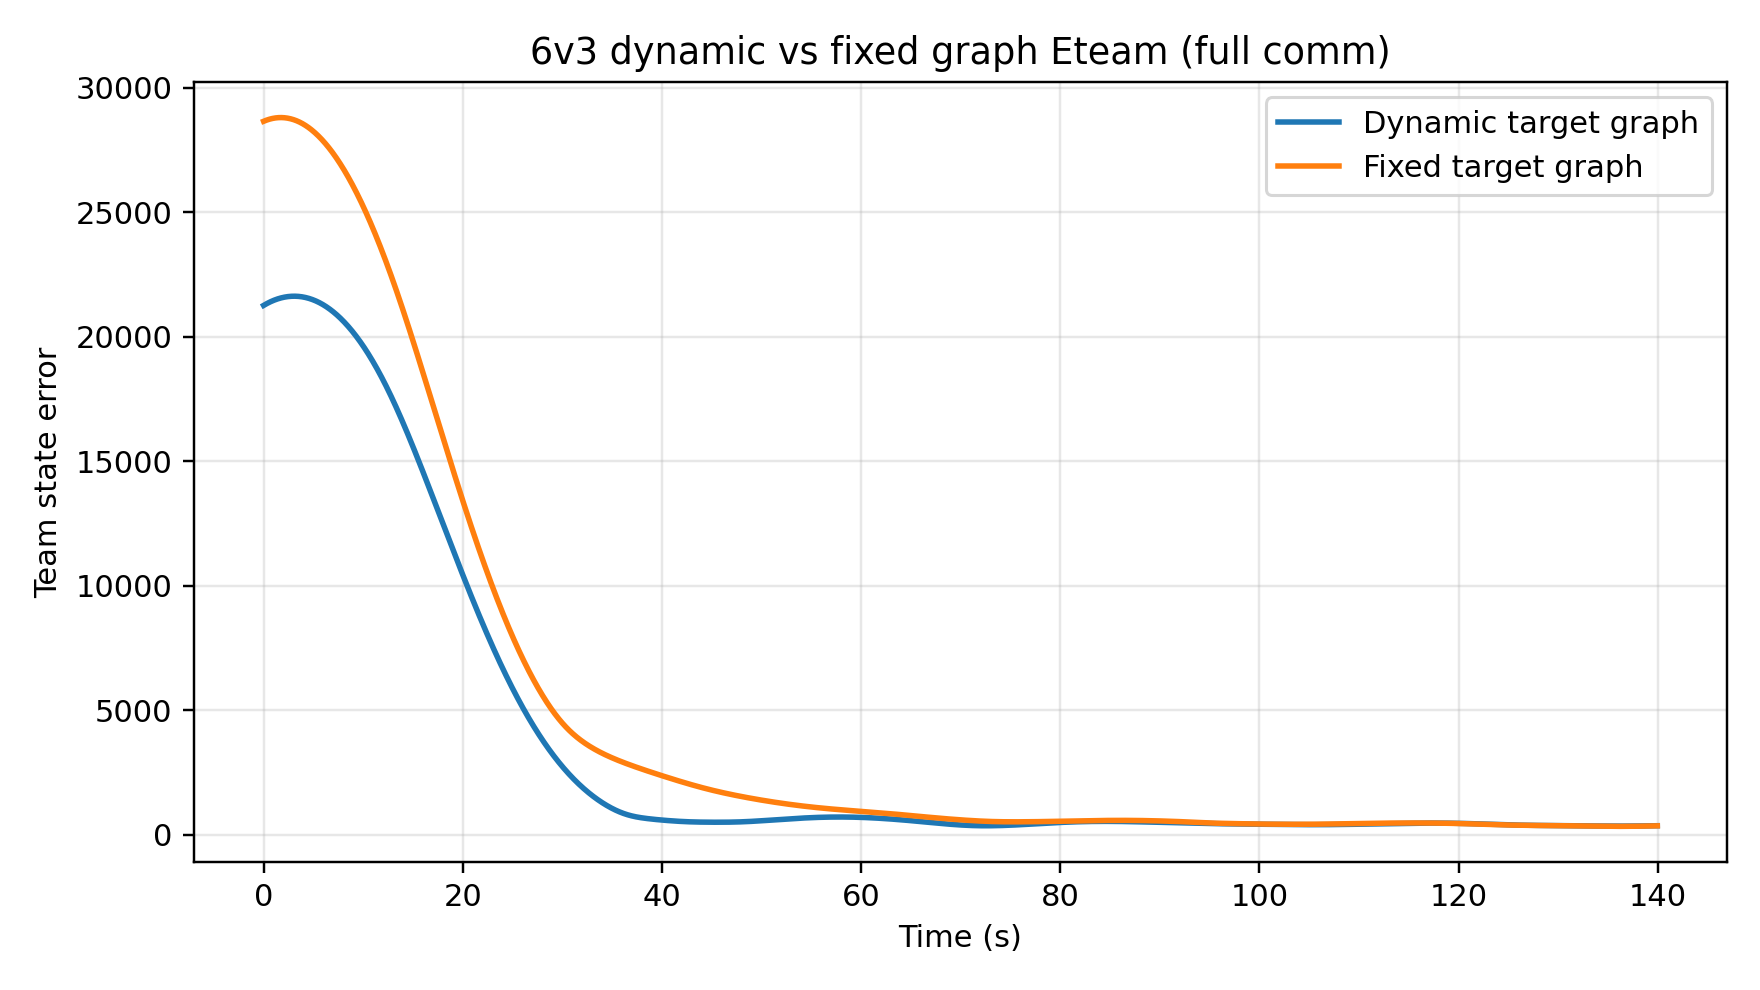
\includegraphics[width=\linewidth]{paper_figures/fig_team_error_6v3.png}}
\caption{6追3团队状态误差：动态目标图（蓝）vs 固定图（橙）。动态分配始终降低团队误差。}
\label{fig:team_6v3}
\end{figure}


\subsection{场景三：三追三（对照组）}

\begin{figure}[htbp]
\centerline{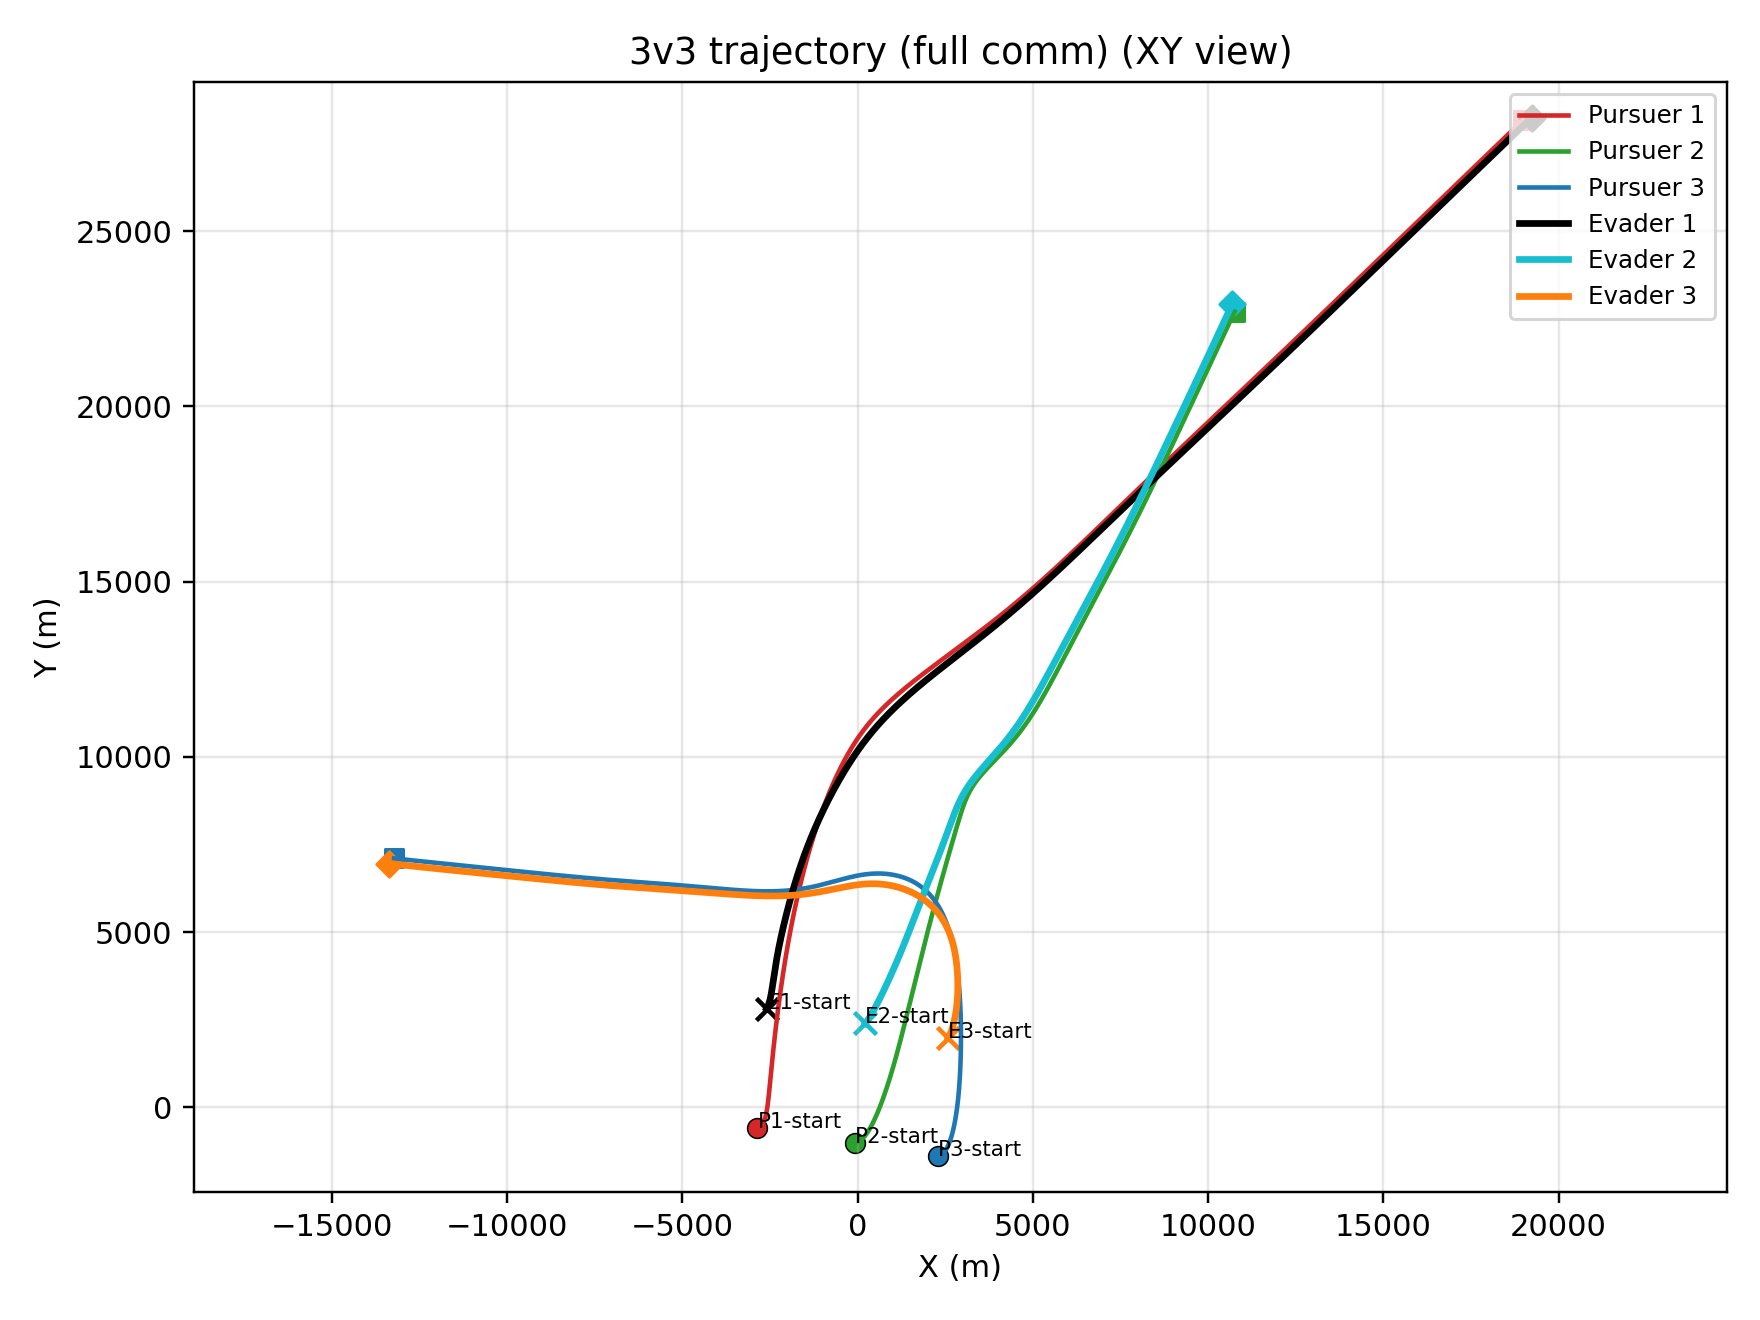
\includegraphics[width=\linewidth]{paper_figures/fig_trajectory_3v3.png}}
\caption{3追3轨迹。每个逃逸者被一个智能体追踪；通信图无组内边，三种模式结果完全相同。}
\label{fig:traj_3v3}
\end{figure}

3追3充当天然对照实验。$N_p/N_e = 1$时，每个逃逸者仅被一个智能体追踪，组内通信图无边（$d_j = 0$），协调梯度恒为零。图~\ref{fig:traj_3v3}展示追逐几何，表~\ref{tab:results}确认三种模式产生相同捕获时间（33.5秒），验证了协调机制在无组内邻居时被正确禁用。


\subsection{Critic权重收敛}

\begin{figure}[htbp]
\centerline{
\includegraphics[width=\linewidth]{paper_figures/fig_weight_convergence.png}}
\caption{6追3的critic权重收敛（$\|\hat{W}_{j,s}\|^2$）。衰减学习率产生自然的平台。}
\label{fig:convergence}
\end{figure}

图~\ref{fig:convergence}绘制了6追3训练过程中$\|\hat{W}_{j,s}\|^2$的变化。衰减学习率$\alpha_s = 0.05 \times 0.85^s$产生从快速调整到稳定平台的平滑过渡。由于训练使用$\gamma = 0$，收敛行为与基线V-SNAC完全相同。


% =====================================================================
\section{结论}
% =====================================================================

本文提出了一种面向非线性动力学与执行器饱和约束下多追逐者追逃博弈的通信增广控制策略。
核心思想是在饱和控制律内部将基于排斥的协调梯度叠加到值函数梯度上，打破由解耦逐追逐者优化所导致的轨迹退化。
该方法仅需通过组内通信图交换位置信息，不改变训练过程，且在通信不可用时自动恢复为标准策略。

在非线性六自由度飞行器模型上的仿真表明，协调机制使接近轨迹多样化，同时保持捕获性能——在某些配置下甚至略有改善。方法在30\%丢包下性能变化可忽略不计。受控场景确认基线在对称追击条件下产生完全重合的路径，而协调梯度消除了这一退化。

未来工作将研究基于实时邻近度的自适应协调强度调度、向异构智能体动力学的推广，以及显式的通信延迟建模。


\begin{thebibliography}{25}

\bibitem{b_isaacs}
R.~Isaacs, \emph{Differential Games}. New York: Dover, 1999.

\bibitem{b_chen2016}
J.~Chen, W.~Zha, Z.~Peng, and D.~Gu, ``Multi-player pursuit--evasion games with one superior evader,'' \emph{Automatica}, vol.~71, pp.~24--32, 2016.

\bibitem{b_yan2022}
R.~Yan, Z.~Shi, and Y.~Zhong, ``Cooperative pursuit-evasion games with a superior evader,'' \emph{Annu. Rev. Control}, vol.~53, pp.~32--51, 2022.

\bibitem{b_zhang2023}
R.~Zhang, Q.~Zong, X.~Zhang, L.~Dou, and B.~Tian, ``Game of drones: Multi-UAV pursuit-evasion game with online motion planning by deep reinforcement learning,'' \emph{IEEE Trans. Neural Netw. Learn. Syst.}, vol.~34, no.~10, pp.~7900--7909, 2023.

\bibitem{b_gong2020}
H.~Gong, S.~Gong, and J.~Li, ``Pursuit--evasion game for satellites based on continuous thrust reachable domain,'' \emph{IEEE Trans. Aerosp. Electron. Syst.}, vol.~56, no.~6, pp.~4626--4637, 2020.

\bibitem{b_shishika2020}
D.~Shishika and V.~Kumar, ``Local-game decomposition for multiplayer perimeter-defense problem,'' in \emph{Proc. IEEE CDC}, 2020, pp.~2093--2098.

\bibitem{b_lopez2020}
V.~G. Lopez, F.~L. Lewis, Y.~Wan, E.~N. Sanchez, and L.~Fan, ``Solutions for multiagent pursuit-evasion games on communication graphs: Finite-time capture and asymptotic behaviors,'' \emph{IEEE Trans. Autom. Control}, vol.~65, no.~5, pp.~1911--1923, 2020.

\bibitem{b_lewis1998}
F.~Lewis, S.~Jagannathan, and A.~Yesildirak, \emph{Neural Network Control of Robot Manipulators and Non-Linear Systems}. New York: Taylor \& Francis, 1998.

\bibitem{b_vsnac_ref}
Z.~Xu, D.~Yu, Y.-J. Liu, and Z.~Wang, ``Approximate optimal strategy for multiagent system pursuit--evasion game,'' \emph{IEEE Syst. J.}, vol.~18, no.~3, pp.~1671--1681, 2024.

\bibitem{b_graphswap}
W.~Lin, Z.~Qu, and M.~A. Simaan, ``Nash strategies for pursuit-evasion differential games involving limited observations,'' \emph{IEEE Trans. Aerosp. Electron. Syst.}, vol.~51, no.~2, pp.~1347--1356, 2015.

\bibitem{b_maddpg}
R.~Lowe, Y.~Wu, A.~Tamar, J.~Harb, P.~Abbeel, and I.~Mordatch, ``Multi-agent actor-critic for mixed cooperative-competitive environments,'' in \emph{Proc. NeurIPS}, 2017, pp.~6379--6390.

\bibitem{b_commrl2025}
Z.~Peng, G.~Wu, B.~Luo, and L.~Wang, ``Multi-UAV cooperative pursuit strategy with limited visual field in urban airspace: A MARL approach,'' \emph{IEEE/CAA J. Autom. Sinica}, vol.~12, no.~7, 2025.

\bibitem{b_icao_separation}
International Civil Aviation Organization, ``Procedures for air navigation services---air traffic management,'' ICAO Doc 4444, 16th ed., 2016.

\bibitem{b_collision_uav}
S.~Feng, L.~Liu, Y.~Yang, and W.~Song, ``Multi-UAVs collaborative path planning in the cramped environment,'' \emph{IEEE/CAA J. Autom. Sinica}, vol.~11, no.~2, pp.~348--363, 2024.

\bibitem{b_ren2005}
W.~Ren and R.~W. Beard, ``Consensus seeking in multiagent systems under dynamically changing interaction topologies,'' \emph{IEEE Trans. Autom. Control}, vol.~50, no.~5, pp.~655--661, 2005.

\bibitem{b_olfati2004}
R.~Olfati-Saber and R.~M. Murray, ``Consensus problems in networks of agents with switching topology and time-delays,'' \emph{IEEE Trans. Autom. Control}, vol.~49, no.~9, pp.~1520--1533, 2004.

\bibitem{b_graphgame2023}
K.~Zhang, Z.~Yang, and T.~Ba\c{s}ar, ``Multi-agent reinforcement learning: A selective overview of theories and algorithms,'' in \emph{Handbook of RL and Control}. Springer, 2021, pp.~321--384.

\bibitem{b_ames2017}
A.~D. Ames, X.~Xu, J.~W. Grizzle, and P.~Tabuada, ``Control barrier function based quadratic programs for safety critical systems,'' \emph{IEEE Trans. Autom. Control}, vol.~62, no.~8, pp.~3861--3876, 2017.

\bibitem{b_zhou2024}
H.~Zhou \emph{et al.}, ``Optimal pursuit strategies for multi-pursuer single-evader games based on cooperative tracking,'' \emph{Optim. Control Appl. Methods}, vol.~45, no.~3, pp.~1234--1250, 2024.

\bibitem{b_formrl2024}
Y.~Li \emph{et al.}, ``Reinforcement learning-based formation-surrounding control for multiple quadrotor UAVs pursuit-evasion games,'' \emph{ISA Trans.}, vol.~146, pp.~180--195, 2024.

\bibitem{b_jagat2017}
A.~Jagat and A.~J. Sinclair, ``Nonlinear control for spacecraft pursuit-evasion game using the state-dependent Riccati equation method,'' \emph{IEEE Trans. Aerosp. Electron. Syst.}, vol.~53, no.~6, pp.~3032--3042, 2017.

\bibitem{b_shi2021}
Z.~Shi, M.~Xu, and Q.~Pan, ``4-D flight trajectory prediction with constrained LSTM network,'' \emph{IEEE Trans. Intell. Transp. Syst.}, vol.~22, no.~11, pp.~7242--7255, 2021.

\bibitem{b_wangj2020}
J.~Wang, C.~Wang, Y.~Wei, and C.~Zhang, ``Neuroadaptive sliding mode formation control of autonomous underwater vehicles with uncertain dynamics,'' \emph{IEEE Syst. J.}, vol.~14, no.~3, pp.~3325--3333, 2020.

\bibitem{b_safety2025}
Y.~Gao, T.~Zhang, and H.~Li, ``Reinforcement learning in pursuit-evasion differential game: Safety, stability and robustness,'' \emph{arXiv:2507.19516}, 2025.

\bibitem{b_huang2024}
X.~Huang and H.~Xu, ``Differential graphical games of multiagent systems with nonzero leader's control input and external disturbances,'' \emph{Int. J. Robust Nonlinear Control}, vol.~34, no.~9, pp.~6055--6076, 2024.

\end{thebibliography}

\end{document}
